\documentclass[12pt]{article}

\usepackage[table]{xcolor}

\usepackage[hidelinks]{hyperref}
\usepackage{etoolbox}
\usepackage{graphicx}
\usepackage{adjustbox}

\makeatletter
\def\ScaleIfNeeded{%
  \ifdim\Gin@nat@width>\linewidth
    \linewidth
  \else
    \Gin@nat@width
  \fi
}
\makeatother

% fonts
\usepackage[T1]{fontenc}
\usepackage[utf8]{inputenc}
\usepackage{textgreek}
\usepackage[greek,english]{babel}
\usepackage{amsmath}

% Code highlight and colors
\usepackage{listings}
\lstset{
  numbers=left,
  tabsize=1,
  basicstyle=\small\ttfamily,
  breaklines=true
}

\usepackage{booktabs, tabularx, longtable}
\usepackage{csquotes}
\usepackage{authblk}

% Geometry block
\usepackage[letterpaper]{geometry}
\providecommand{\tightlist}{\setlength{\itemsep}{0pt}\setlength{\parskip}{0pt}}

\title{Data-based, synthesis-driven: setting the agenda for computational
ecology}

\author[1,2,3]{Timothée~Poisot}
\author[1,2]{Richard~LaBrie}
\author[4]{Erin~Larson}
\author[5]{Anastasia~Rahlin}
\author[6,7]{Benno I.~Simmons}
\affil[1]{Université de Montréal, Département de Sciences Biologiques}
\affil[2]{Groupe de Recherche Interuniversitaire en Limnologie et environnement
aquatique}
\affil[3]{Québec Centre for Biodiversity Sciences}
\affil[4]{Department of Ecology and Evolutionary Biology, Cornell University}
\affil[5]{Illinois Natural History Survey}
\affil[6]{Conservation Science Group, Department of Zoology, University of
Cambridge, Cambridge, UK}
\affil[7]{Department of Animal and Plant Sciences, University of Sheffield,
Sheffield, UK}

\begin{document}

\maketitle

\begin{abstract}
  Computational thinking is the integration of algorithms, software, and
  data, to solve general questions in a field. Computation ecology has the
  potential to transform the way ecologists think about the integration of
  data and models. As the practice is gaining prominence as a way to
  conduct ecological research, it is important to reflect on what its
  agenda could be, and how it fits within the broader landscape of
  ecological research. In this contribution, we suggest areas in which
  empirical ecologists, modellers, and the emerging community of
  computational ecologists could engage in a constructive dialogue to
  build on one another's expertise; specifically, about the need to make
  predictions from models actionable, about the best standards to
  represent ecological data, and about the proper ways to credit data
  collection and data reuse. We discuss how training can be amended to
  improve computational literacy.
\end{abstract}

% pandoc-xnos: cleveref fakery
\newcommand{\plusnamesingular}{}
\newcommand{\starnamesingular}{}
\newcommand{\xrefname}[1]{\protect\renewcommand{\plusnamesingular}{#1}}
\newcommand{\Xrefname}[1]{\protect\renewcommand{\starnamesingular}{#1}}
\providecommand{\cref}{\plusnamesingular~\ref}
\providecommand{\Cref}{\starnamesingular~\ref}
\providecommand{\crefformat}[2]{}
\providecommand{\Crefformat}[2]{}

% pandoc-xnos: cleveref formatting
\crefformat{figure}{fig.~#2#1#3}
\Crefformat{figure}{Figure~#2#1#3}
\crefformat{equation}{eq.~#2#1#3}
\Crefformat{equation}{Equation~#2#1#3}
\crefformat{table}{table~#2#1#3}
\Crefformat{table}{Table~#2#1#3}

Computational science happens when algorithms, software, data management
practices, and advanced research computing are put in interaction with
the explicit goal of solving \enquote{complex} problems. Typically,
problems are considered complex when they cannot be solved appropriately
with mathematical modelling (defined here as the application of
mathematical models that are not explicitly grounded into empirical
data) or data-collection only (Dörner \& Funke 2017). Computational
science is the application of computational thinking to research
questions (Papert 1996), \emph{i.e.} the feedback loop of abstracting a
problem to its core mechanisms, expressing a solution in a way that can
be automated, and using interactions between simulations and data to
refine the original problem or suggest new knowledge. Computational
approaches are commonplace in most areas of biology, to the point where
one would almost be confident that they represent a viable career path
(Bourne 2011). Collecting ecological data is a time-consuming, costly,
and demanding project; in addition, the variability of these data is
high (both in terms of variance and in terms of quantity and
completeness). In parallel, many ecological problems lack appropriate
formal mathematical formulations, which we need in order to construct
strong, testable hypotheses. For these reasons, computational approaches
hold great possibilities, notably to further ecological synthesis and
assist decision-making (Petrovskii \& Petrovskaya 2012).

Levin (2012) suggested that ecology (and evolutionary biology) should
continue their move towards a \emph{marriage of theory and data}. In
addition to the lack of adequately expressed models, this effort is
hampered by the fact that data and models are often developed by
different groups of scientists, and reconciling both can be difficult.
This has been suggested as one of the reasons for why theoretical papers
(defined as \emph{papers with at least one equation in the main text})
experience a lower number of citations (Fawcett \& Higginson 2012); this
is the tragic sign that empirical scientists either do not see the value
of theoretical work, or have not received the training to usefully rely
on math-heavy theoretical papers, which of course can be blamed on both
parties. One of the leading textbooks on mathematical models in ecology
and evolution (Otto \& Day 2007) is more focused with algebra and
calculus, and not with the integration of models with data. Other
manuals that cover the integration of models and data tend to lean more
towards statistical models (Bolker 2008; Soetaert \& Herman 2008). This
paints a picture of ecology as a field in which dynamical models and
empirical data do not interact much, and instead the literature develops
in silos.

Computational ecology is the application of computational science to
ecological problems. This defines three core characteristics of
computational ecology. First, it recognizes ecological systems as
complex and adaptive; this places a great emphasis on mathematical tools
that can handle, or even require, a certain degree of stochasticity to
accommodate or emulate what is found in nature (Zhang 2010, 2012).
Second, it understands that data are the final arbiter of any simulation
or model (Petrovskii \& Petrovskaya 2012); this favours the use of
data-driven approaches and analyses (Beaumont 2010). On this point,
computational approaches differ greatly from the production of
theoretical models able to stand on their own with no data input.
Finally, it accepts that some ecological systems are too complex to be
formulated in mathematical or programmatic terms (Pascual 2005); the use
of conceptual, or \enquote{toy} models, as long as they can be
confronted to empirical data, is preferable to \enquote{abusing}
mathematics by describing the wrong mechanism well (May 2004). By
contrast, modelling approaches are, by construction, limited to problems
that can be expressed in mathematical terms. To summarize, we define
computational ecology as the sub-field tasked with integrating
real-world data with mathematical, conceptual, and numerical models (if
possible by deeply coupling them), in order to assist with the
most-needed goal of improving the predictive accuracy of ecological
research and synthesising ecological knowledge (Houlahan et al. 2017;
Maris et al. 2017). Jørgensen (2008) identified that one of the current
challenges is to facilitate the integration of existing data in the
explosion of modelling techniques (most of which were designed to answer
long-standing questions in ecological research).

Ecology as a whole (and community ecology in particular) circumvented
the problem of model and data mismatch by investing in the development
and refinement of statistical models (see Warton et al. 2014 for an
excellent overview) and \enquote{numerical} approaches (Legendre \&
Legendre 1998) based on multivariate statistics. These models are able
to \emph{explain} data, but very rarely do they give rise to new
predictions -- despite it being a very clear priority even if we
\enquote{simply} seek to further our understanding (Houlahan et al.
2017). Computational ecology can fill this niche; at the cost of a
higher degree of abstraction, its integration of data and generative
models (\emph{i.e.} models that, given rules, will generate new data)
can be helpful to initiate the investigation of questions that have not
received (or perhaps cannot receive) extensive empirical treatment, or
for which usual statistical approaches fall short. In particular, we
argue that computational approaches can serve a dual purpose. First,
they can deliver a more predictive science, because they are explicitly
data-driven. Second, they can guide the attention of researchers towards
mechanisms of interest; in a context where time and resources are
finite, and the urgency to understand ecological systems is high, this
may be the main selling point of computational techniques.

In a thought-provoking essay, Markowetz (2017) suggests that \emph{all
biology is computational biology} -- the rationale behind this bold
statement being that integrating computational advances, novel
mathematical tools, and the usual data from one field, has a high
potential to deliver synthesis. A more reasonable statement would be
that \emph{all ecology can benefit from computational ecology}, as long
as we can understand how it interacts with other approaches; in this
paper, we attempt to situate the practice of computational ecology
within the broader scope of ecological research. The recent years have
given us an explosion of new tools, training opportunities, and
mechanisms for data access. One can assume that computational approaches
will become more tempting, and more broadly adopted. This requires us to
address the questions of the usefulness and promises of this line of
research, as well as the caveats associated with it. In particular, we
highlight the ways in which computational ecology differs from, and
complements, ecological modelling that does not involve data directly.
We finally move on to the currency of collaborations between different
sub-disciplines of ecologists, and discuss the need to add more
quantitative skills in ecological training and to develop a culture
where specialising in computational research is accepted.

Advancing ecology through computational techniques is an ongoing work,
and has already delivered many results (some of which we discuss in the
text). To elevate this approach, the community of practising ecologists
needs to establish baselines of appropriate practices for the sharing
and re-use of existing data, especially when they are massively
aggregated and re-purposed; reach a consensus on a common core of
training which enables students to explore computational approaches in
addition to more usual approaches. Ultimately, a better integration of
computational techniques in the practice of ecological research has the
potential to improve transparency and reproducibility, and facilitate
the synthesis of ecological knowledge.

\hypertarget{a-success-story-species-distribution-models}{%
\section{A success story: Species Distribution
Models}\label{a-success-story-species-distribution-models}}

The practice known as \enquote{species distribution modelling} (and the
species distribution models, henceforth SDMs, it generates) is a good
example of computational practices generating novel ecological insights.
At their core, SDMs seek to model the presences or absences of a species
based on previous observations of its presences or absences, and
knowledge of the environment in which the observations were made. More
formally, SDMs can be interpreted as having the form \(\text{P}(S | E)\)
(or \(\text{P}(S=1 | E)\) for presence-only models), where \(S\) denotes
the presence of a species, and \(E\) is an array of variables
representing the local state of the environment at the point where the
prediction is made (the location is represented, not by its spatial
positions, but by a suite of environmental variables).

As Franklin (2010) highlights, SDMs emerged at a time where access to
computers \emph{and} the ability to effectively program them became
easier. Although ecological insights, statistical methods, and data
already existed, the ability to turn these ingredients into something
predictive required what is now called \enquote{computational literacy}
-- the ability to abstract and automate a system to generate predictions
through computer simulations and their validation. One of the strengths
of SDMs is that they can be used either for predictions or explanations
of where a given species occur (Elith \& Leathwick 2009) and can be
corroborated with empirical data. To calculate \(\text{P}(S | E)\) is to
make a prediction (what is the likelihood of observing species \(S\) at
a given location), that can be refined, validated, or rejected based on
cross-validation (Hijmans 2012) or \emph{de novo} field sampling (West
et al. 2016). To understand \(E\), \emph{i.e.} the environmental aspects
that determine species presence, is to form an explanation of a
distribution that relates to the natural history of a species.

SDMs originated as statistical and correlative models, and are now
incorporating more ecological theory (Austin 2002) -- being able to
integrate (abstract) ideas and knowledge with (formal) statistical and
numerical tools is a key feature of computational thinking. In fact, one
of the most recent and most stimulating developments in the field of
SDMs is to refine their predictions not through the addition of more
data, but through the addition of more processes (Franklin 2010). These
SDMs rely on the usual statistical models, but also on dynamical models
(for example simulations; \emph{e.g.} Wisz et al. (2012) or Pellissier
et al. (2013) for biotic interactions, and Miller \& Holloway (2015) for
movement and dispersal). What they lack in mathematical expressiveness
(\emph{i.e.} having a closed-form solution (Borwein \& Crandall 2013),
which is often ruled out by the use of stochastic models or agent-based
simulations), they assume to gain in predictive ability through the
explicit consideration of more realistic ecological mechanisms (D'Amen
et al. 2017; Staniczenko et al. 2017).

SDMs have been a success, but there are many other areas of ecology that
could be improved by a marriage of computational ecology and empirical
data. The novel use of genomic RNA-seq data and existing
\passthrough{\lstinline!worldclim!} climate data allowed the creation of
random forest models in order to make predictions of where yellow
warbler populations, a species of conservation concern, are most
vulnerable to climate change (Bay et al. 2018). Environmental DNA
metabarcoding data coupled with machine learning approaches and linear
models was used to create, test, and predict biodiversity indices for
benthic foraminifera, which can be applied to monitoring health of fish
farm ecosystems (Cordier et al. 2017). The increase in data volume,
coupled with access to computing techniques and power, will result in a
multiplication of these boundary-pushing studies in the next years.

\hypertarget{outlining-computational-ecology}{%
\section{Outlining computational
ecology}\label{outlining-computational-ecology}}

Most research approaches exist on a gradient. In this section, we will
outline research practices which differ enough in their approaches to
fall under the umbrella of computational science, and specifically
discuss how they can provide novel information. We will first show how
computational ecology complements other research approaches, then
discuss how it can be used in the current context to facilitate
interactions between theoretical and empirical research.

\hypertarget{computational-ecology-in-focus}{%
\subsection{Computational ecology in
focus}\label{computational-ecology-in-focus}}

The specific example of predator-prey interactions should be a familiar
illustration of how the same problem can be addressed through a variety
of research approaches (\xrefname{fig.}\cref{fig:concept}). The classic
predator--prey equations of Lotka \& Volterra are an instance of a
\enquote{modelling} based perspective, wherein mathematical analysis
reveals how selected parameters (rates of interactions and growth)
affect an ecologically-relevant quantity (population stability and
coexistence). These models, although they have been formulated to
explain data generated through empirical observations, are disconnected
from the data themselves. In fact, this family of model lies at the
basis of a branch of ecological modelling that now exists entirely
outside of data (Ackland \& Gallagher 2004; Gyllenberg et al. 2006;
Coville \& Frederic 2013). These purely mathematical models are often
used to describe trends in time series. But not all of them hold up to
scrutiny when explicitly compared to empirical data. Gilpin (1973)
famously reports that based on the predictions of the Lotka-Volterra
model, hares in the Hudson bay are feeding on Lynx -- this example goes
to show that applying models that have not been validated could be
dangerous, and their output should be framed in the context of external
data.

By contrast Sallan et al. (2011) study the same issue (sustained
persistence and fluctuations of predator--prey couples through time)
using a paleo-ecological timeseries, and interpret their data in the
context of predictions from the Lotka-Volterra family of models (namely,
they find support for Lotka-Volterra-like oscillations in time).
Although dynamical models and empirical data interact in this example,
they do not do so directly; that is, the analysis of empirical data is
done within the context of a broad family of model, but not coupled to
\emph{e.g.} additional simulations. The two are done \emph{in parallel},
and not so much \emph{in interaction}. A number of other models have
been shown to generate predictions that quantitatively match empirical
data (Nicholson \& Bailey 1935; Beverton \& Holt 1957) -- this
represents, in our opinion, the sole test of whether a mathematical
model is adapted to a particular problem and system. While models are
undeniably useful to make mechanisms interact in a low-complexity
setting, it is a grave mistake to assume they will, in and of
themselves, be relevant to empirical systems.

\begin{figure}
\centering
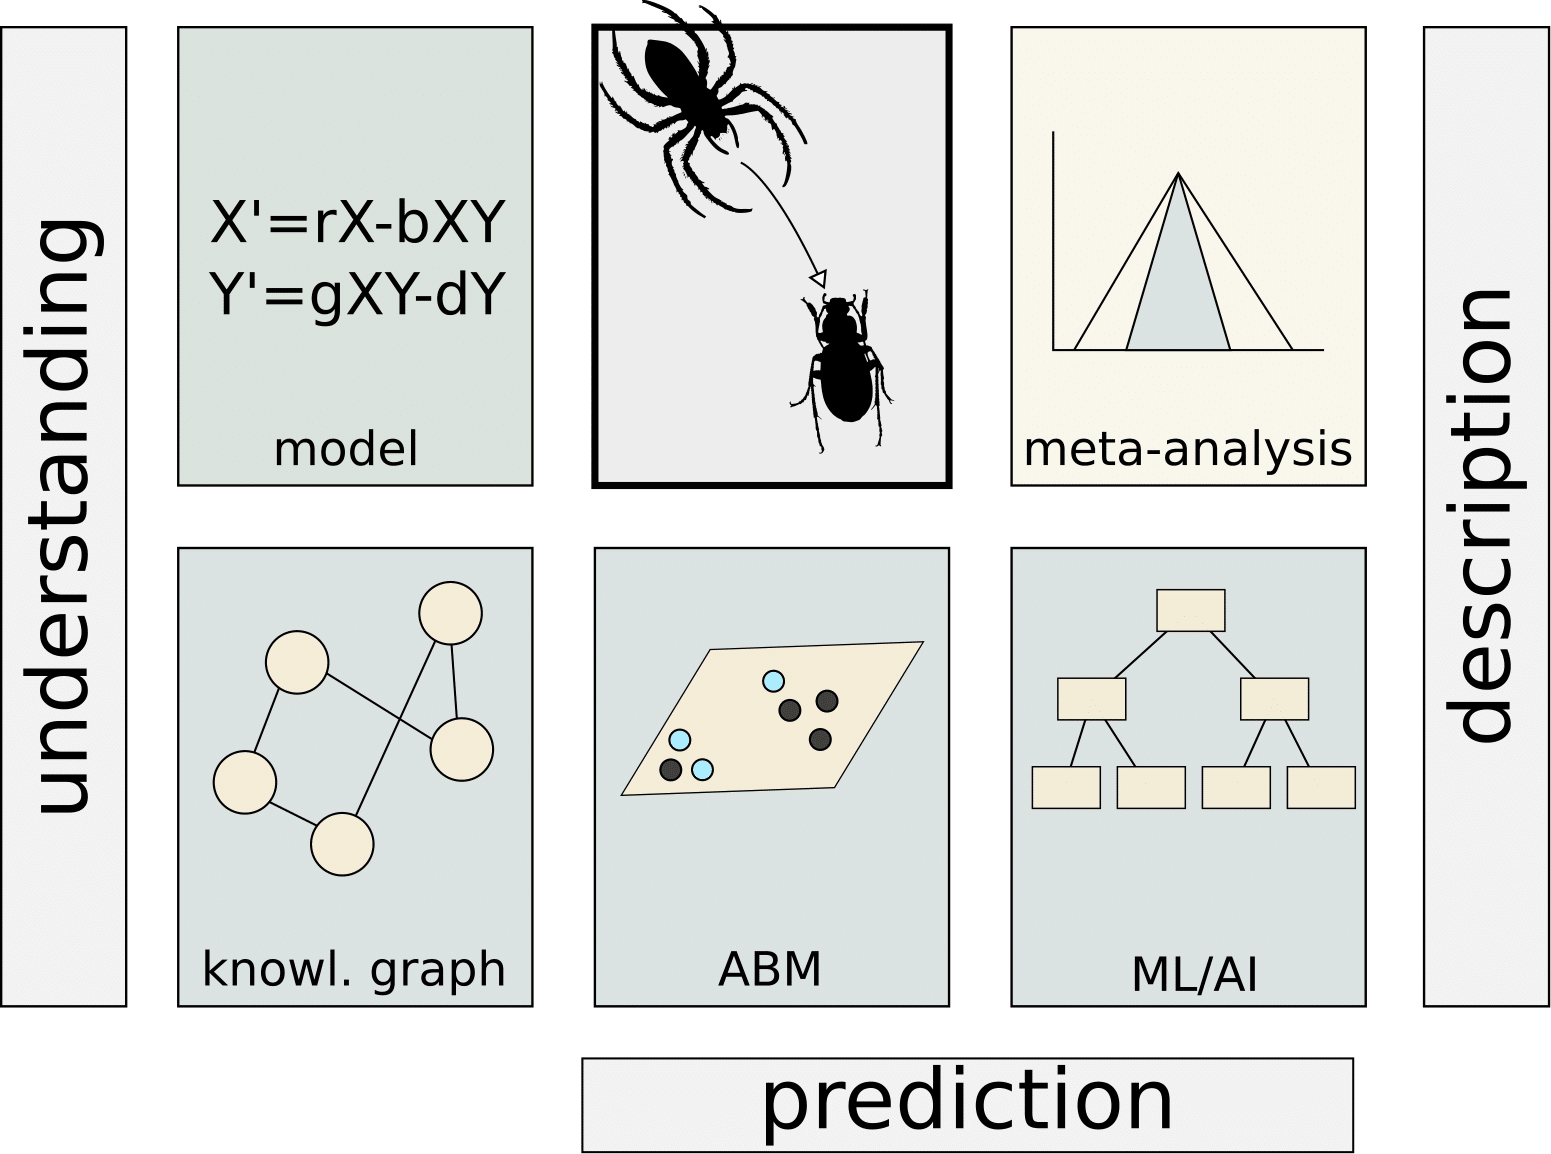
\includegraphics{figures/concept.png}
\caption{An overview of how computational approaches can complement
other research approaches. On the top line, we have represented
empirical studies (center) as well as modelling (left) and meta-analysis
(right; represented as a funnel plot) approaches. In the bottom line, we
have represented three possible approaches to study predator-prey
relationships: knowledge graphs can represent interactions between the
concepts; agent-based modelling can provide some predictions about the
future of the system; methods from machine learning can assist both in
understanding and prediction. Importantly, the goal of these approaches
should always be to return to empirical data.\label{fig:concept}}
\end{figure}

Meta-analyses, such as the one by Bolnick \& Preisser (2005), are
instead interested in collecting the outcome of observational and
manipulative studies, and synthesizing the \emph{effects} they report.
These are often purely \emph{statistical}, in that they aggregate
significance and effect size, to measure how robust a result is across
different systems. Meta-analyses most often require a \emph{critical
mass} of pre-existing papers (Lortie et al. 2013). Although they are
irreplaceable as a tool to measure the strength of results, they are
limited by their need for primary literature with experimental designs
that are sufficiently similar to be comparable.

Predator-prey (and other biotic) interactions have been studied with a
few computational approaches to date. Colon et al. (2015) show how an
agent-based model can guide the interpretation of the same system
represented as ordinary differential equations. This is an important
result, as it offers suggestions to bridge families of models -- not
only can agent-based approaches provide answers about the biological
systems of interest, they can also provide information about the
behaviour of other families of models. Although this example is
primarily model-driven, there are a number of data-driven approaches
that rely on computational techniques. One example is the prediction of
species interactions. Stock et al. (2017) suggested linear filtering to
identify false-negatives (\emph{i.e.} interactions that exist, but may
have been missed) in an empirical dataset. This can guide sampling in
the field, and is to an extent a predictive task, but cannot inform our
understanding of the system. Similarly, Desjardins-Proulx et al. (2017a)
used various recommender systems to infer the prey items of predators
based on knowledge of (i) diet and (ii) functional traits. This results
in testable predictions, but is not necessarily increasing our
understanding of the rules involved in the system.

Chen et al. (2016) used symbolic regression to infer a differential
equations model \emph{from data} about predator-prey interactions. This
is a fascinating result, as it shows just how much signal is contained
in data: enough to describe a mathematical model explaining their
behaviour. And while understanding mechanisms by looking at a time
series may be difficult, understanding the mechanisms when studying
equations dictated by the data themselves is feasible. In a similar
vein, Desjardins-Proulx et al. (2017b) suggest that logic networks,
which describe the relationships between concepts, can be inferred by
optimizing a knowledge bank on the data. This category of approaches
offer the opportunity to increase our understanding of empirical data,
not by thinking deeply about the rules, but by extracting the rules from
the data.

\hypertarget{computational-ecology-in-context}{%
\subsection{Computational ecology in
context}\label{computational-ecology-in-context}}

In \emph{Life on the Mississippi}, Mark Twain wrote that \enquote{There
is something fascinating about science. One gets such wholesale returns
of conjecture out of such a trifling investment of fact}. This is a good
description of the purpose of computational ecology: in a data-limited
context, merging phenomenological models with pre-existing datasets is a
way to efficiently develop conjectures, or more appropriately, build on
our knowledge of models and data to put forward testable, quantified
hypotheses. Perretti et al. (2013) intriguingly report that model-free
inference based on data \emph{always} outperforms the best model: in
other words, we do not understand ecological systems as well as we
think, and approaches putting the data first might always outperform
those relying on expert knowledge. Pascual (2005) outlined that
computational ecology has a unique ability to go from the complex
(natural systems) to the simple (representations and conceptual models),
and back (testable predictions). Although the natural world is immensely
complex, it is paradoxically the high degree of model abstraction in
computational approaches that gives them generality across several
systems. In the years since this article was published, the explosion in
machine learning tools and their predictive ability, and their adoption
by ecologists (Thessen 2016) should have changed the situation quite
significantly.

Yet, with the exception of a still-narrow family of problems that can be
addressed by remote-sensing or meta-genomics, there has been no regime
shift in the rate at which ecological data are collected. Observations
from citizen science accumulate, but are highly biased by societal
preferences rather than conservation priority (Donaldson et al. 2016;
Troudet et al. 2017), by proximity to urban centers and infrastructure
(Geldmann et al. 2016), \emph{as well as} by the interaction between
these factors (Tiago et al. 2017). In addition, Lindenmayer \& Likens
(2018) raise the significant concern that the \enquote{culture} of
ecology must be maintained -- even in the context of a sudden (though
debatable) avalanche of data, ecology as a field should always put
robust hypotheses \emph{first}. This is especially true since our needs
for testable and actionable predictions increased dramatically. This
provides a clear mission statement for computational ecology: refining
the models and further integrating them with data is necessary, and
using methods that work well on reduced amounts of heterogeneous data
must be part of this effort. Enthusiastic reports about the big data
revolution coming to ecology (Hampton et al. 2013; Soranno \& Schimel
2014) have been premature at best, and the challenge associated with
most of our datasets being decidedly \emph{tiny} cannot be easily
dismissed.

Yet data, even small, are \enquote{unreasonably effective} (Halevy et
al. 2009) -- they can reveal trends and signal that may not be
immediately apparent from causal modelling alone, for example.
Ecological models make, by definition, high-accuracy predictions, but
they tend to be difficult to test (Rykiel 1996) -- models relying on
precise mathematical expressions can be difficult to calibrate or
parameterize. Observations (field sampling) or manipulative approaches
(micro/meso/macro-cosms, field experiments) are highly accurate (but
have also immense human and monetary costs that limit the scale at which
they can be applied). There is simply too much nature around for us to
observe, monitor, and manipulate it all. Computational approaches able
to generalize some rules from the data (Desjardins-Proulx et al. 2017a,
2017b) may help guide the attention of researchers onto mechanisms that
are worthy of a deeper investigation. Computational approaches will more
likely shine \emph{in support} to more established areas of research.

Recent advances in computational epidemiology (reviewed in Marathe \&
Ramakrishnan 2013) provide an interesting roadmap for computational
ecology: there have been parallel advances in (i) adapting data
acquisition to maximize the usefulness of novel data analyses methods,
(ii) integration of novel analytical methods from applied mathematics
\emph{and} social sciences, mostly related to computations on large
graphs, to work on pre-existing data, and (iii) a tighter integration of
models to data fluxes to allow near real-time monitoring and prediction.
All of these things are possible in ecological research. In fact, recent
examples (Bush et al. 2017; Harris et al. 2017; Dietze et al. 2018;
White et al. 2018) suggest that near real-time forecasting of
biodiversity is becoming feasible, and is identified by computational
ecologists as a key priority.

\hypertarget{en-route-towards-synthesis}{%
\section{En route towards synthesis}\label{en-route-towards-synthesis}}

Ecological synthesis, usually defined as the integration of data and
knowledge to increase scope, relevance, or usability of results both
across and within sub-fields (Carpenter et al. 2009), is an essential
first step to achieve policy relevance (Baron et al. 2017). Most of the
global policy challenges have an ecological or environmental component,
and outside of the socio-ecological, socio-economical, socio-cultural,
aspects, ecologists can contribute to the mitigation or resolution of
these challenges by i) assessing our knowledge of natural systems, ii)
developing methods to produce scenarios using state-of-the-art models
and tools, and iii) communicating the output of these scenarios to
impact policy-making. White et al. (2015) propose that this falls under
the umbrella of \emph{action ecology}, \emph{i.e.} using fundamental
knowledge and ecological theory to address pressing, real-world
questions.

Raghavan et al. (2016) suggest that this approach can also accommodate
stakeholder knowledge and engagement. By building models that rely on
ecological concepts, empirical data, and stakeholder feedback, they
propose a \emph{computational agroecology} program, to use computational
tools in the optimization of sustainable agricultural practices. This
example suggests that not only can computational approaches yield
fundamental research results in a short time frame, they can also be
leveraged as a tool for applied research and knowledge transfer now. The
definition of \enquote{a short time} is highly sensitive to the context
-- some predictions can be generated using routine tools (in a matter of
weeks), whereas some require the development of novel methodologies, and
may require years. Accelerating the time to prediction will, in large
part, require the development of software that can be deployed and run
more rapidly. Computational ecology is nevertheless nimble enough that
it can be used to iterate rapidly over a range of scenarios, to inform
interactions with policy makers or stakeholders in near real time. We
need to mention that there is a lower bound on time to prediction: some
applications require different degrees of accuracy. While an approximate
result is good enough for fundamental research, outputs used to enact
policy making that can affect thousands of citizens (and change the
dynamics of a region or an ecosystem) require a better accuracy. The
variety of computational techniques allows moving across these scales,
while the advances in programming practices and computing power
decreases the severity of the accuracy/runtime tradeoff.

\hypertarget{mapping-the-domains-of-collaboration}{%
\subsection{Mapping the domains of
collaboration}\label{mapping-the-domains-of-collaboration}}

Understanding how computational ecology will fit within the broader
research practices requires answering three questions: what can
computational ecology bring to the table, what are the needs of
computational ecologists, and what are the current limitations of
computational approaches that could limit their immediate applicability.
It seems, at this point, important to minimize neither the importance
nor the efficiency of sampling and collection of additional data.
Sampling is important because ecological questions, no matter how
fundamental, ought to be grounded in phenomena happening in nature, and
these are revealed by observation or manipulation of natural systems.
Sampling is efficient because it is the final arbiter: how good any
prediction is at explaining aspects of a particular empirical system is
determined by observations of this system, compared to the predictions.

Relying heavily on external information implies that computational
research is dependent on standards for data representation. The
Ecological Metadata Language (Fegraus et al. 2005) is an attempt at
standardizing the way meta-data are represented for ecological data;
adherence to this standard, although it has been shown to improve the
ease of assembling large datasets from single studies (Gil et al. 2011),
is done on a voluntary basis (and its uptake is therefore abysmal). An
alternative approach is to rely on community efforts to pre-curate and
pre-catalog ecological data, such as with the flagship effort
\emph{EcoDataRetriever} (Morris \& White 2013). Yet even this approach
is ultimately limited because of the human factor involved --- when the
upstream data change, they have to be re-worked into the software. A
community consensus on data representation, although unlikely, would
actually solve several problems at once. First, it would make the
integration of multiple data sources trivial. Second, it would provide
clear guidelines about the input and storage of data, thus maybe
improving their currently limited longevity (Vines et al. 2014).
Finally, it would facilitate the integration of data and models with
minimum efforts and risk of mis-communication, since the format would be
the same for all. To this extent, a recent proposal by Ovaskainen et al.
(2017) is particularly interesting: rather than deciding on formats
based on knowledge of eco-informatics or data management best practices,
why not start from the ecological concepts, and translate them in
digital representation? The current way to represent \emph{e.g.}
biodiversity data has largely been designed based on the needs of
collection managers, and bears little to no relevance to most extant
research needs. Re-designing the way we store and manipulate data based
on research practices is an important step forward, and will ultimately
benefit researchers. To be generalized, this task requires a strong
collaboration between ecologists with topic expertise, ecologists with
field expertise, and those of us leaning closest to the computational
part of the field.

With or without a common data format, the problem remains that we have
very limited insights into how error in predictions made on synthetic
datasets will propagate from an analysis to another (Poisot et al.
2016); in a succession of predictive steps, do errors at each step
amplify, or cancel one another? Biases exist in the underlying data and
in the models used to generate the predictions, and these biases can
manifest in three possible outcomes. First, predictions from these
datasets accumulate bias and cannot be used. Second, because the scale
at which these predictions are expressed is large, errors are
(quantitatively) small enough to be over-ridden by the magnitude of
actual variation. Finally, in the best-case but low-realism scenario,
errors end up cancelling each other out. The best possible way to
understand how errors propagate is to validate predictions \emph{de
novo}, through sampling. Model-validation methods can be used, as they
are with SDMs (Hijmans 2012), but \emph{de novo} sampling carries the
additional weight of being an independent attempt at testing the
prediction. Improved collaborations on this aspect will provide
estimates of the robustness of the predictions, in addition to
highlighting the steps of the process in which uncertainty is high ---
these steps are natural candidates for additional methodological
development.

Finally, there is a need to assess how the predictions made by purely
computational approaches will be fed back into other types of research.
This is notably true when presenting these approaches to stakeholders.
One possible way to make this knowledge transfer process easier is to be
transparent about the way predictions were derived: which data were used
(with citations for credits and unique identifiers for reproducibility),
which software was used (with versions numbers and code), and what the
model / simulations do (White et al. 2013). In short, the onus is on
practitioners of computational research to make sure we provide all the
information needed to communicate how predictions came to be.

\hypertarget{establishing-the-currencies-of-collaboration}{%
\subsection{Establishing the currencies of
collaboration}\label{establishing-the-currencies-of-collaboration}}

An important question to further the integration of computational
approaches to the workflow of ecological research is to establish
\emph{currencies} for collaborations. Both at the scale of individual
researchers, research group, and larger research communities, it is
important to understand what each can contribute to the research effort.
As ecological research is expected to be increasingly predictive and
policy-relevant, and as fundamental research tends to tackle
increasingly refined and complex questions, it is expected that research
problems will become more difficult to resolve. This is an incentive for
collaborations that build on the skills that are specific to different
approaches.

In an editorial to the \emph{New England Journal of Medicine}, Longo \&
Drazen (2016) characterized scientists using previously published data
as \enquote{research parasites} (backlash by a large part of the
scientific community caused one of the authors to later retract the
statement -- Drazen (2016)). Although community ecologists would have,
anyways, realized that the presence of parasites indicates a healthy
ecosystem (Marcogliese 2005; Hudson et al. 2006), this feeling of unfair
benefit for ecological data re-analysis (Mills et al. 2015) has to be
addressed, because it has no empirical support. The rate of data re-use
in ecology is low and has a large delay (Evans 2016), and there are no
instances of re-analysing existing data for the same (or similar)
purpose they were produced for. There is a necessary delay between the
moment data are available, and the moment where they are aggregated and
re-purposed (especially considering that data are, at the earliest,
published at the same time as the paper). This delay is introduced by
the need to understand the data, see how they can be combined, develop a
research hypothesis, etc..h

On the other hand, there are multiple instances of combining multiple
datasets collected at different scales to address an entirely different
question (see GBIF 2016 for an excellent showcase) -- it is more likely
that data re-use is done with the intent of exploring different
questions. It is also worth remembering that ecology as a whole, and
macroecology and biogeography in particular, already benefit immensely
from data re-use. For example, data collected by citizen scientists are
used to generate estimates of biodiversity distribution, but also set
and refine conservation targets (Devictor et al. 2010); an overwhelming
majority of our knowledge of bird richness and distribution comes from
the \emph{eBird} project (Sullivan et al. 2009, 2014), which is
essentially fed by the unpaid work of citizen scientists.

With this in mind, there is no tip-toeing around the fact that
computational ecologists will be \emph{data consumers}, and this data
will have to come from ecologists with active field programs (in
addition to government, industry, and citizens). Recognizing that
computational ecology \emph{needs} these data as a condition for its
continued existence and relevance should motivate the establishment of a
way to credit and recognize the role of \emph{data producers} (which is
discussed in Poisot et al. 2016, in particular in the context of massive
dataset aggregation). Data re-users must be extremely pro-active in the
establishment of crediting mechanisms for data producers; as the
availability of these data is crucial to computational approaches, and
as we do not share any of the cost of collecting these data, it behooves
us to make sure that our research practices do not accrue a cost for our
colleagues with field or lab programs. Encouraging conversations between
data producers and data consumers about what data will be shared, when,
and how databases will be maintained will improve both collaborations
and research quality. In parallel, data producers can benefit from the
new analytical avenues opened by advances in computational ecology.
Research funders should develop financial incentives to these
collaborations, specifically by dedicating a part of the money to
developing and implementing sound data archival and re-use strategies,
and by encouraging researchers to re-use existing data when they exist.

\hypertarget{training-data-minded-ecologists}{%
\subsection{Training data-minded
ecologists}\label{training-data-minded-ecologists}}

The fact that data re-use is not instantaneously convenient reveals
another piece of information about computational ecology: it relies on
different skills, and different tools than those typically used by field
ecologists. One of the most fruitful avenues for collaboration lies in
recognizing the strengths of different domains: the skills required to
assemble a dataset (taxonomic expertise, natural history knowledge,
field know-how) and the skills required to develop robust computational
studies (programming, applied mathematics) are different. Because these
skills are so transversal to any form of ecological research, we are
confident that they can be incorporated in any curriculum. If anything,
this calls for increased collaboration, where these approaches are put
to work in complementarity.

Barraquand et al. (2014) highlighted the fact that professional
ecologists received \emph{less} quantitative and computational thinking
that they think should be necessary. Increasing the amount of such
training does not necessarily imply that natural history or field
practice will be sacrificed on the altar of mathematics: rather, ecology
would benefit from introducing more quantitative skills and reasoning
across all courses, and introductory ones in particular (Hoffman et al.
2016). Instead of dividing the field further between empirically and
theoretically-minded scientists, this would showcase quantitative skills
as being transversal to all questions that ecology can address. What to
teach, and how to integrate it to the existing curriculum, does of
course require discussion and consensus building by the community.

A related problem is that most practising ecologists are terrible role
models when it comes to showcasing good practices of data management
(because there are no incentives to do this); and data management is a
crucial step towards easier computational approaches. Even in the
minority of cases where ecologists do share their data on public
platforms, there are so few metadata that not being able to reproduce
the original study is the rule (Roche et al. 2014, 2015). This is a
worrying trend, because data management affects how easily research is
done, regardless of whether the data are ultimately archived. Because
the volume and variety of data we can collect tends to increase over
time, and because we expect higher standards of analysis (therefore
requiring more programmatic approaches relying on the use or development
of purpose-specific code), data management has already became a core
skill for ecologists to acquire.

This view is echoed in recent proposals. Mislan et al. (2016) suggested
that highlighting the importance of code in most ecological studies
would be a way to bring the community to adopt higher standards, all the
while de-mystifying the process of producing code. As with increased
mandatory data release alongside more reproducible publication
requirements by funding agencies, mandatory code release would benefit a
more reproducible science and show how data were transformed during the
analysis. This also requires teaching ecologists how to evaluate the
quality of the software they use~(Poisot 2015). Finally, Hampton et al.
(2015) proposed that the \enquote{Tao of Open Science} would be
particularly beneficial to the entire field of ecology; as part of the
important changes in attitude, they identified the solicitation and
integration of productive feedback throughout the research process.
Regardless of the technical solution, this emphasizes the need to
foster, in ecologists in training, a culture of discussion across
disciplinary boundaries.

All of these points can be distilled into practical training
recommendations for different groups in the community of ecologists.
Classes based around lab or field experience should emphasize practical
data management skills which have been validated as best practices by
the community (Soyka et al. 2017), and introduce tools that would make
the maintenance of data easier. Modelling classes, especially when
concerned about purely mathematical models, should add modules on the
way these models can be integrated with empirical data. Finally,
computational classes should emphasize communication skills: what do
these new tools do, and how can they be used by other fields in ecology;
but also, how do we properly track citations to data, and give credit to
data producers? Building these practices into training would ensure that
the next generation of ecologists will be able to engage in a meaningful
dialogue across methodological boundaries.

\hypertarget{fostering-a-culture-of-mutual-respect-and-acceptance}{%
\subsection{Fostering a culture of mutual respect and
acceptance}\label{fostering-a-culture-of-mutual-respect-and-acceptance}}

While the origins of ecology are grounded in field research, the growth
of computational ecology has been accompanied by an increasing segment
of ecologists who do not, or have never, conducted fieldwork.
Anecdotally, this new class of researcher has caused some tensions
between computational ecologists and field ecologists, at the level of
individuals, mixed-method research groups and the ecological community
at large. Expectations of fieldwork are also sometimes embedded
institutionally, such as with hiking equipment as prizes in ecological
competitions.

Part of these tensions may be driven by a view of computational
ecologists as \enquote{research parasites}, and this is another reason
to develop crediting mechanisms for data producers, as discussed above.
However, tensions are sometimes also predicated on two sequential
assumptions: (i) that computational ecologists have less affinity for
the natural world and/or less natural history knowledge of the systems
they work in; and (ii) that these deficits reduce the ability of
computational ecologists to carry out sound ecological science.

Whether the first assumption is true will vary widely among individuals.
However, it is important to note that interest in ecological research
and enjoyment of outdoor pursuits are not necessarily collinear, and
that computational skills do not preclude natural history knowledge.
Assumption two is both incorrect and unhelpful. Such views must be
addressed because they may negatively affect ecology as a discipline.
For example, people in disciplines like mathematics or physics, who may
have superb quantitative skills but little interest in field work, may
be less likely to become ecologists or to work with field ecologists,
despite the potential to make profound contributions. Similarly, those
who do not carry out fieldwork due to physical or mental disability,
medical conditions, or simply personal preference, should not be made to
feel as though they are unable to make valid scientific contributions.
Criticizing, or ridiculing, the work or choices of early-career/student
computational ecologists could be particularly damaging. It is important
to note that such tensions may run the other way, and it is essential
too for computational ecologists to recognize that field ecologists make
irreplaceable contributions, whether possessing advanced quantitative
skills or not.

Ultimately, it is necessary for ecology to foster a culture where
methodological specialization is accepted. The importance of field
knowledge -- such as sampling and natural history -- is undoubtedly
important, as is advanced quantitative and computational knowledge. That
different individuals may hold these skills should motivate
collaboration, not hostility. Such changes are urgently needed for
computational ecology to flourish with, rather than alongside, field
ecology.

\hypertarget{concluding-remarks}{%
\section{Concluding remarks}\label{concluding-remarks}}

None of the theoretical, mathematical, computational approaches to
ecological research have any intrinsic superiority -- in the end, direct
observation and experimentation trumps all, and serve as the validation,
rejection, or refinement of predictions derived in other ways, but lacks
the scaling power to be the only viable solution. The growing
computational power, growing amount of data, and increasing
computational literacy in ecology means that producing theory and
predictions is becoming cheaper and faster (regardless of the quality of
these products). Yet the time needed to test any prediction is not
decreasing (or at least not as fast). Computational science has resulted
in the development of many tools and approaches that can be useful to
ecology, since they allow ecologists of all kinds to wade through these
predictions and data. Confronting theoretical predictions to data is a
requirement, if not the core, of ecological synthesis; this is only
possible under the conditions that ecologists engage in meaningful
dialogue across disciplines, and recognize the currencies of their
collaborations.

Discussing the place of computational ecology within the broader context
of the ecological sciences will highlight areas of collaborations with
other areas of science. Thessen (2016) makes the point that
long-standing ecological problems would benefit from being examined
through a variety of machine learning techniques -- We fully concur,
because these techniques usually make the most of existing data (Halevy
et al. 2009). Reaching a point where these methods are routinely used by
ecologists will require a shift in our culture: quantitative training is
currently perceived as inadequate (Barraquand et al. 2014), and most
graduate programs do not train ecology students in contemporary
statistics (Touchon \& McCoy 2016).

Ultimately, any additional data collection has its scope limited by
financial, human, and temporal constraints --- or in other words, we
need to chose what to sample, because we can't afford to sample it all.
Computational approaches, because they can work through large amounts of
data, and integrate them with models that can generate predictions,
might allow answering an all important question: what do we sample, and
where? Some rely on their ecological intuition to answer; although
computational ecologists may be deprived of such intuitions, they have
the know-how to couple data and models, and can meaningfully contribute
to this answer. Computational ecology is also remarkably cost-effective.
Although the reliance on advanced research computing incurs immense
costs (including hardware maintenance, electrical power, and training of
highly qualified personnel; these are often absorbed by local or
national consortia), it allows the generation of predictions that are
highly testable. Although the accuracy of these predictions is currently
unknown (and will vary on a model/study/question basis), any additional
empirical effort to \emph{validate} predictions will improve their
quality, reinforcing the need for dialogue and collaborations.

\textbf{Acknowledgements:} TP thanks Dr.~Allison Barner and Dr.~Andrew
McDonald for stimulating discussions, and the Station de Biologie des
Laurentides de l'Université de Montréal for hosting him during part of
the writing process. TP thanks the Canadian Institute for Ecology and
Evolution for financial support. BIS is supported by the Natural
Environment Research Council as part of the Cambridge Earth System
Science NERC DTP (NE/L002507/1). We thank the volunteers of Software
Carpentry and Data Carpentry, whose work contribute to improving the
skills of ecologists. Carabid picture by Maxime Dahirel (CC-BY 4.0),
spider image by Sidney Frederic Harmer, Arthur Everett Shipley,
digitized by Maxime Dahirel (CC-BY 4.0).

\hypertarget{references}{%
\section*{References}\label{references}}
\addcontentsline{toc}{section}{References}

\hypertarget{refs}{}
\leavevmode\hypertarget{ref-AcklGall04}{}%
\textbf{Ackland \& Gallagher}. (2004). Stabilization of Large
Generalized Lotka-Volterra Foodwebs By Evolutionary Feedback. \emph{Phys
Rev Lett.} 93.

\leavevmode\hypertarget{ref-Aust02}{}%
\textbf{Austin}. (2002). Spatial prediction of species distribution: an
interface between ecological theory and statistical modelling.
\emph{Ecological Modelling.} 157:101--18.

\leavevmode\hypertarget{ref-BaroSpec17}{}%
\textbf{Baron et al.} (2017). Synthesis Centers as Critical Research
Infrastructure. \emph{BioScience.}

\leavevmode\hypertarget{ref-BarrEzar14}{}%
\textbf{Barraquand et al.} (2014). Lack of quantitative training among
early-career ecologists: a survey of the problem and potential
solutions. \emph{PeerJ.} 2:e285.

\leavevmode\hypertarget{ref-BayHarr18}{}%
\textbf{Bay et al.} (2018). Genomic signals of selection predict
climate-driven population declines in a migratory bird. \emph{Science.}
359:83--6.

\leavevmode\hypertarget{ref-Beau10}{}%
\textbf{Beaumont}. (2010). Approximate Bayesian Computation in Evolution
and Ecology. \emph{Annu Rev Ecol Evol Syst.} 41:379--406.

\leavevmode\hypertarget{ref-BeveHolt57}{}%
\textbf{Beverton \& Holt}. (1957). On the dynamics of exploited fish
populations. Springer Science \& Business Media;

\leavevmode\hypertarget{ref-Bolk08}{}%
\textbf{Bolker}. (2008). Ecological models and data in R. Princeton
University Press;

\leavevmode\hypertarget{ref-BolnPrei05}{}%
\textbf{Bolnick \& Preisser}. (2005). Resource competition modifies the
strength of trait-mediated predator--prey interactions: a meta-analysis.
\emph{Ecology.} 86:2771--9.

\leavevmode\hypertarget{ref-BorwCran13}{}%
\textbf{Borwein \& Crandall}. (2013). Closed Forms: What They Are and
Why We Care. \emph{Not Am Math Soc.} 60:50.

\leavevmode\hypertarget{ref-Bour11}{}%
\textbf{Bourne}. (2011). Ten Simple Rules for Getting Ahead as a
Computational Biologist in Academia. \emph{PLoS Comput Biol.}
7:e1002001.

\leavevmode\hypertarget{ref-BushSoll17}{}%
\textbf{Bush et al.} (2017). Connecting Earth observation to
high-throughput biodiversity data. \emph{Nat Ecol Evol.}
1:s41559--017--0176--017.

\leavevmode\hypertarget{ref-CarpArmb09}{}%
\textbf{Carpenter et al.} (2009). Accelerate Synthesis in Ecology and
Environmental Sciences. \emph{BioScience.} 59:699--701.

\leavevmode\hypertarget{ref-ChenAngu16}{}%
\textbf{Chen et al.} (2016). Revealing complex ecological dynamics via
symbolic regression. \emph{bioRxiv.}:074617.

\leavevmode\hypertarget{ref-ColoClae15}{}%
\textbf{Colon et al.} (2015). Bifurcation analysis of an agent-based
model for predator--prey interactions. \emph{Ecol Model.} 317:93--106.

\leavevmode\hypertarget{ref-CordEsli17}{}%
\textbf{Cordier et al.} (2017). Predicting the Ecological Quality Status
of Marine Environments from eDNA Metabarcoding Data Using Supervised
Machine Learning. \emph{Environ Sci Technol.} 51:9118--26.

\leavevmode\hypertarget{ref-CoviFred13}{}%
\textbf{Coville \& Frederic}. (2013). Convergence To The Equilibrium In
A Lotka-Volterra Ode Competition System With Mutations. \emph{arXiv.}

\leavevmode\hypertarget{ref-DAmMate17}{}%
\textbf{D'Amen et al.} (2017). Improving spatial predictions of
taxonomic, functional and phylogenetic diversity. \emph{J Ecol.}

\leavevmode\hypertarget{ref-DesjLaig17}{}%
\textbf{Desjardins-Proulx et al.} (2017a). Ecological interactions and
the Netflix problem. \emph{PeerJ.} 5.

\leavevmode\hypertarget{ref-DesjPois17}{}%
\textbf{Desjardins-Proulx et al.} (2017b). Scientific Theories and
Artificial Intelligence. \emph{bioRxiv.}:161125.

\leavevmode\hypertarget{ref-DeviWhit10}{}%
\textbf{Devictor et al.} (2010). Beyond scarcity: citizen science
programmes as useful tools for conservation biogeography. \emph{Divers
Distrib.} 16:354--62.

\leavevmode\hypertarget{ref-DietFox18}{}%
\textbf{Dietze et al.} (2018). Iterative near-term ecological
forecasting: Needs, opportunities, and challenges.
\emph{PNAS.}:201710231.

\leavevmode\hypertarget{ref-DonaBurn16}{}%
\textbf{Donaldson et al.} (2016). Taxonomic bias and international
biodiversity conservation research. \emph{FACETS.}

\leavevmode\hypertarget{ref-DornFunk17}{}%
\textbf{Dörner \& Funke}. (2017). Complex Problem Solving: What It Is
and What It Is Not. \emph{Front Psychol.} 8.

\leavevmode\hypertarget{ref-Draz16}{}%
\textbf{Drazen}. (2016). Data Sharing and the Journal. \emph{N Engl J
Med.} 374:e24.

\leavevmode\hypertarget{ref-ElitLeat09}{}%
\textbf{Elith \& Leathwick}. (2009). Species Distribution Models:
Ecological Explanation and Prediction Across Space and Time. \emph{Annu
Rev Ecol Evol Syst.} 40:677--97.

\leavevmode\hypertarget{ref-Evan16}{}%
\textbf{Evans}. (2016). Gauging the Purported Costs of Public Data
Archiving for Long-Term Population Studies. \emph{PLOS Biol.}
14:e1002432.

\leavevmode\hypertarget{ref-FawcHigg12}{}%
\textbf{Fawcett \& Higginson}. (2012). Heavy use of equations impedes
communication among biologists. \emph{PNAS.} 109:11735--9.

\leavevmode\hypertarget{ref-FegrAnde05}{}%
\textbf{Fegraus et al.} (2005). Maximizing the Value of Ecological Data
with Structured Metadata: An Introduction to Ecological Metadata
Language (EML) and Principles for Metadata Creation. \emph{Bull Ecol Soc
Am.} 86:158--68.

\leavevmode\hypertarget{ref-Fran10a}{}%
\textbf{Franklin}. (2010). Mapping species distributions: spatial
inference and prediction. Cambridge University Press;

\leavevmode\hypertarget{ref-GBIF16}{}%
\textbf{GBIF}. 2016 Oct. GBIF Science Review 2016 {[}Internet{]}.

\leavevmode\hypertarget{ref-GeldHeil16}{}%
\textbf{Geldmann et al.} (2016). What determines spatial bias in citizen
science? Exploring four recording schemes with different proficiency
requirements. \emph{Diversity Distrib.} 22:1139--49.

\leavevmode\hypertarget{ref-Gilp73}{}%
\textbf{Gilpin}. (1973). Do Hares Eat Lynx? \emph{Am Nat.} 107:727--30.

\leavevmode\hypertarget{ref-GilVand11}{}%
\textbf{Gil et al.} (2011). Examples of ecological data synthesis driven
by rich metadata, and practical guidelines to use the Ecological
Metadata Language specification to this end. \emph{Int J Metadata Semant
Ontol.} 6:46.

\leavevmode\hypertarget{ref-GyllYan06}{}%
\textbf{Gyllenberg et al.} (2006). Limit cycles for
competitor--competitor--mutualist Lotka--Volterra systems. \emph{Phys
Nonlinear Phenom.} 221:135--45.

\leavevmode\hypertarget{ref-HaleNorv09}{}%
\textbf{Halevy et al.} (2009). The Unreasonable Effectiveness of Data.
\emph{IEEE Intell Syst.} 24:8--12.

\leavevmode\hypertarget{ref-HampAnde15}{}%
\textbf{Hampton et al.} (2015). The Tao of open science for ecology.
\emph{Ecosphere.} 6:1--13.

\leavevmode\hypertarget{ref-HampStra13}{}%
\textbf{Hampton et al.} (2013). Big data and the future of ecology.
\emph{Front Ecol Environ.} 11:156--62.

\leavevmode\hypertarget{ref-HarrTayl17}{}%
\textbf{Harris et al.} (2017). Forecasting biodiversity in breeding
birds using best practices. \emph{bioRxiv.}:191130.

\leavevmode\hypertarget{ref-Hijm12}{}%
\textbf{Hijmans}. (2012). Cross-validation of species distribution
models: removing spatial sorting bias and calibration with a null model.
\emph{Ecology.} 93:679--88.

\leavevmode\hypertarget{ref-HoffLeup16}{}%
\textbf{Hoffman et al.} (2016). Development and Assessment of Modules to
Integrate Quantitative Skills in Introductory Biology Courses.
\emph{Cell Biol Educ.} 15:ar14--4.

\leavevmode\hypertarget{ref-HoulMcKi17}{}%
\textbf{Houlahan et al.} (2017). The priority of prediction in
ecological understanding. \emph{Oikos.} 126:1--7.

\leavevmode\hypertarget{ref-HudsDobs06}{}%
\textbf{Hudson et al.} (2006). Is a healthy ecosystem one that is rich
in parasites? \emph{Trends Ecol Evol.} 21:381--5.

\leavevmode\hypertarget{ref-Jorg08}{}%
\textbf{Jørgensen}. (2008). Overview of the model types available for
development of ecological models. \emph{Ecological Modelling.} 215:3--9.

\leavevmode\hypertarget{ref-LegeLege98}{}%
\textbf{Legendre \& Legendre}. (1998). Numerical ecology. Oxford, UK:
Elsevier;

\leavevmode\hypertarget{ref-Levi12}{}%
\textbf{Levin}. (2012). Towards the marriage of theory and data.
\emph{Interface Focus.} 2:141--3.

\leavevmode\hypertarget{ref-LindLike18}{}%
\textbf{Lindenmayer \& Likens}. (2018). Maintaining the culture of
ecology. \emph{Front Ecol Environ.} 16:195--5.

\leavevmode\hypertarget{ref-LongDraz16}{}%
\textbf{Longo \& Drazen}. (2016). Data Sharing. \emph{N Engl J Med.}
374:276--7.

\leavevmode\hypertarget{ref-LortStew13}{}%
\textbf{Lortie et al.} 2013 Jun. Practical interpretation of ecological
meta-analyses {[}Internet{]}. PeerJ PrePrints; Report No.: e38v1.

\leavevmode\hypertarget{ref-MaraRama13}{}%
\textbf{Marathe \& Ramakrishnan}. (2013). Recent Advances in
Computational Epidemiology. \emph{IEEE Intell Syst.} 28:96--101.

\leavevmode\hypertarget{ref-Marc05}{}%
\textbf{Marcogliese}. (2005). Parasites of the superorganism: Are they
indicators of ecosystem health? \emph{Int J Parasitol.} 35:705--16.

\leavevmode\hypertarget{ref-MariHune17}{}%
\textbf{Maris et al.} (2017). Prediction in ecology: promises, obstacles
and clarifications. \emph{Oikos.}:n/a--a.

\leavevmode\hypertarget{ref-Mark17}{}%
\textbf{Markowetz}. (2017). All biology is computational biology.
\emph{PLOS Biology.} 15:e2002050.

\leavevmode\hypertarget{ref-May04}{}%
\textbf{May}. (2004). Uses and Abuses of Mathematics in Biology.
\emph{Science.} 303:790--3.

\leavevmode\hypertarget{ref-MillHoll15}{}%
\textbf{Miller \& Holloway}. (2015). Incorporating movement in species
distribution models. \emph{Prog Phys Geogr.} 39:837--49.

\leavevmode\hypertarget{ref-MillTepl15}{}%
\textbf{Mills et al.} (2015). Archiving Primary Data: Solutions for
Long-Term Studies. \emph{Trends Ecol Evol.} 30:581--9.

\leavevmode\hypertarget{ref-MislHeer16}{}%
\textbf{Mislan et al.} (2016). Elevating The Status of Code in Ecology.
\emph{Trends in Ecology \& Evolution.} 31:4--7.

\leavevmode\hypertarget{ref-MorrWhit13}{}%
\textbf{Morris \& White}. (2013). The EcoData Retriever: Improving
Access to Existing Ecological Data. \emph{PLoS ONE.} 8:e65848.

\leavevmode\hypertarget{ref-NichBail35}{}%
\textbf{Nicholson \& Bailey}. (1935). The Balance of Animal
Populations.---Part I. \emph{Proc Zool Soc Lond.} 105:551--98.

\leavevmode\hypertarget{ref-OttoDay07}{}%
\textbf{Otto \& Day}. (2007). A biologist's guide to mathematical
modeling in ecology and evolution. Princeton University Press;

\leavevmode\hypertarget{ref-OvasTikh17}{}%
\textbf{Ovaskainen et al.} (2017). How to make more out of community
data? A conceptual framework and its implementation as models and
software. \emph{Ecol Lett.}:n/a--a.

\leavevmode\hypertarget{ref-Pape96}{}%
\textbf{Papert}. (1996). An exploration in the space of mathematics
educations. \emph{Int J Comput Math Learn.} 1.

\leavevmode\hypertarget{ref-Pasc05}{}%
\textbf{Pascual}. (2005). Computational Ecology: From the Complex to the
Simple and Back. \emph{PLoS Comp Biol.} 1:e18.

\leavevmode\hypertarget{ref-PellRohr13}{}%
\textbf{Pellissier et al.} (2013). Combining food web and species
distribution models for improved community projections. \emph{Ecol
Evol.} 3:4572--83.

\leavevmode\hypertarget{ref-PerrMunc13}{}%
\textbf{Perretti et al.} (2013). Model-free forecasting outperforms the
correct mechanistic model for simulated and experimental data.
\emph{PNAS.} 110:5253--7.

\leavevmode\hypertarget{ref-PetrPetr12}{}%
\textbf{Petrovskii \& Petrovskaya}. (2012). Computational ecology as an
emerging science. \emph{Interface Focus.} 2:241--54.

\leavevmode\hypertarget{ref-Pois15}{}%
\textbf{Poisot}. (2015). Best publishing practices to improve user
confidence in scientific software. \emph{Ideas Ecol Evol.} 8.

\leavevmode\hypertarget{ref-PoisGrav16}{}%
\textbf{Poisot et al.} (2016). Synthetic datasets and community tools
for the rapid testing of ecological hypotheses. \emph{Ecography.}
39:402--8.

\leavevmode\hypertarget{ref-RaghNard16}{}%
\textbf{Raghavan et al.} (2016). Computational Agroecology.
\emph{Proceedings of the 2016 CHI Conference Extended Abstracts on Human
Factors in Computing Systems - CHI EA '16.} Association for Computing
Machinery (ACM);

\leavevmode\hypertarget{ref-RochKruu15}{}%
\textbf{Roche et al.} (2015). Public Data Archiving in Ecology and
Evolution: How Well Are We Doing? \emph{PLOS Biol.} 13:e1002295.

\leavevmode\hypertarget{ref-RochLanf14}{}%
\textbf{Roche et al.} (2014). Troubleshooting Public Data Archiving:
Suggestions to Increase Participation. Eisen, ed. \emph{PLoS Biol.}
12:e1001779.

\leavevmode\hypertarget{ref-Ryki96}{}%
\textbf{Rykiel}. (1996). Testing ecological models: the meaning of
validation. \emph{Ecol Model.} 90:229--44.

\leavevmode\hypertarget{ref-SallKamm11}{}%
\textbf{Sallan et al.} (2011). Persistent predator-prey dynamics
revealed by mass extinction. \emph{Proc Natl Acad Sci.} 108:8335--8.

\leavevmode\hypertarget{ref-SoetHerm08}{}%
\textbf{Soetaert \& Herman}. (2008). A Practical Guide to Ecological
Modelling: Using R as a Simulation Platform. Springer Verlag;

\leavevmode\hypertarget{ref-SoraSchi14}{}%
\textbf{Soranno \& Schimel}. (2014). Macrosystems ecology: big data, big
ecology. \emph{Front Ecol Environ.} 12:3--3.

\leavevmode\hypertarget{ref-SoykBudd17}{}%
\textbf{Soyka et al.} (2017). Using Peer Review to Support Development
of Community Resources for Research Data Management. \emph{J EScience
Librariansh.} 6.

\leavevmode\hypertarget{ref-StanSiva17}{}%
\textbf{Staniczenko et al.} (2017). Linking macroecology and community
ecology: refining predictions of species distributions using biotic
interaction networks. \emph{Ecol Lett.}:n/a--a.

\leavevmode\hypertarget{ref-StocPois17}{}%
\textbf{Stock et al.} (2017). Linear filtering reveals false negatives
in species interaction data. \emph{Sci Rep.} 7:45908.

\leavevmode\hypertarget{ref-SullAycr14}{}%
\textbf{Sullivan et al.} (2014). The eBird enterprise: an integrated
approach to development and application of citizen science. \emph{Biol
Conserv.} 169:31--40.

\leavevmode\hypertarget{ref-SullWood09}{}%
\textbf{Sullivan et al.} (2009). eBird: A citizen-based bird observation
network in the biological sciences. \emph{Biol Conserv.} 142:2282--92.

\leavevmode\hypertarget{ref-Thes16}{}%
\textbf{Thessen}. (2016). Adoption of Machine Learning Techniques in
Ecology and Earth Science. \emph{One Ecosyst.} 1:e8621.

\leavevmode\hypertarget{ref-TiagCeia17}{}%
\textbf{Tiago et al.} (2017). Spatial distribution of citizen science
casuistic observations for different taxonomic groups. \emph{Sci Rep.}
7:12832.

\leavevmode\hypertarget{ref-ToucMcCo16}{}%
\textbf{Touchon \& McCoy}. (2016). The mismatch between current
statistical practice and doctoral training in ecology. \emph{Ecosphere.}
7:e01394.

\leavevmode\hypertarget{ref-TrouGran17}{}%
\textbf{Troudet et al.} (2017). Taxonomic bias in biodiversity data and
societal preferences. \emph{Sci Rep.} 7:9132.

\leavevmode\hypertarget{ref-VineAlbe14}{}%
\textbf{Vines et al.} (2014). The Availability of Research Data Declines
Rapidly with Article Age. \emph{Curr Biol.} 24:94--7.

\leavevmode\hypertarget{ref-WartFost14}{}%
\textbf{Warton et al.} (2014). Model-based thinking for community
ecology. \emph{Plant Ecol.} 216:669--82.

\leavevmode\hypertarget{ref-WestKuma16}{}%
\textbf{West et al.} (2016). Field validation of an invasive species
Maxent model. \emph{Ecological Informatics.} 36:126--34.

\leavevmode\hypertarget{ref-WhitBald13}{}%
\textbf{White et al.} (2013). Nine simple ways to make it easier to
(re)use your data. \emph{Ideas Ecol Evol.} 6.

\leavevmode\hypertarget{ref-WhitSutt15}{}%
\textbf{White et al.} (2015). The next generation of action ecology:
novel approaches towards global ecological research. \emph{Ecosphere.}
6:1--16.

\leavevmode\hypertarget{ref-WhitYenn18}{}%
\textbf{White et al.} (2018). Developing an automated iterative
near-term forecasting system for an ecological study.
\emph{bioRxiv.}:268623.

\leavevmode\hypertarget{ref-WiszPott12}{}%
\textbf{Wisz et al.} (2012). The role of biotic interactions in shaping
distributions and realised assemblages of species: implications for
species distribution modelling. \emph{Biol Rev.} 88:15--30.

\leavevmode\hypertarget{ref-Zhan10}{}%
\textbf{Zhang}. (2010). Computational ecology: artificial neural
networks and their applications. Singapore: World Scientific Publ;

\leavevmode\hypertarget{ref-Zhan12}{}%
\textbf{Zhang}. (2012). Computational ecology: graphs, networks and
agent-based modeling. New Jersey: World Scientific;

\end{document}
